\chapter{Partie site Web}

Afin de réaliser notre projet, nous avons dû créer un site Web pour accueillir toutes les données que l'Arduino aura obtenu grâce au capteur.

\section{Deux technologies : HTML/CSS et PHP}

Pour ce faire, il nous a fallu coder ce site avec le langage HTML pour la partie fixe du site et le langage PHP pour la partie du qui viendra à changer au cours du temps.

\subsection{Partie statique : HTML et CSS}

Pour créer un site Web, il faut le coder à la main\footnote{Ou en passant par un logiciel spécifique.}. Pour cela, il existe deux langages que sont le HTML et le CSS. À l'heure actuelle, le HTML est en version 5 et le CSS en version 3. Le HTML et le CSS sont complémentaires. En effet, le premier nous sert pour le fond, c'est-à-dire le contenu ; le second pour la forme, l'apparence.

Le HTML est un langage balistique : il utilise des balises de la forme \verb-<balise>- et \verb-</balise>-. Il est donc très compréhensible. Voici un exemple de page HTML :
\FichierCode{HTML}{Codes/HTML-CSS/Exemple.html}

\Espace

D'un autre côté, le CSS s'organise en propriétés, en classes et en identificateurs. Il est capable de mettre en forme le HTML. Pour associer une classe ou un identificateur à une balise, il suffit d'utiliser respectivement les arguments \verb/class="ma-class"/ et \verb/id="mon-identificateur"/ sur une balise quelconque. Contrairement à une classe, un identificateur ne peut s'utiliser qu'une fois dans une page. Dans le fichier CSS, les classes sont précédées d'un point, les identificateurs d'un croisillon \verb-#- et leurs propriétés sont entre accolades.

Supposons un fichier CSS nommé \verb-style.css- avec le contenu suivant.
\FichierCode{CSS}{Codes/HTML-CSS/Exemple.css}
À partir de cela, nous pouvons créer un fichier HTML utilisant ces classes.
\FichierCode{HTML}{Codes/HTML-CSS/Exemple_CSS.html}
Ainsi, nous pouvons voir le résultat sur la figure suivante.

\begin{figure}[!h]
	\centering
	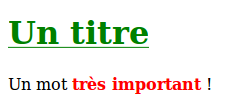
\includegraphics[width=.2\linewidth]{Images/Exemple_CSS}
	\caption{Exemple de CSS}
\end{figure}

Notre site est alors constitué de ces deux langages. Vous pouvez en voir un aperçu sur la figure suivante ou en ligne sur \url{http://tpe.teguad.ovh}.

\begin{figure}[!h]
	\begin{minipage}{.5\linewidth}
		\centering
		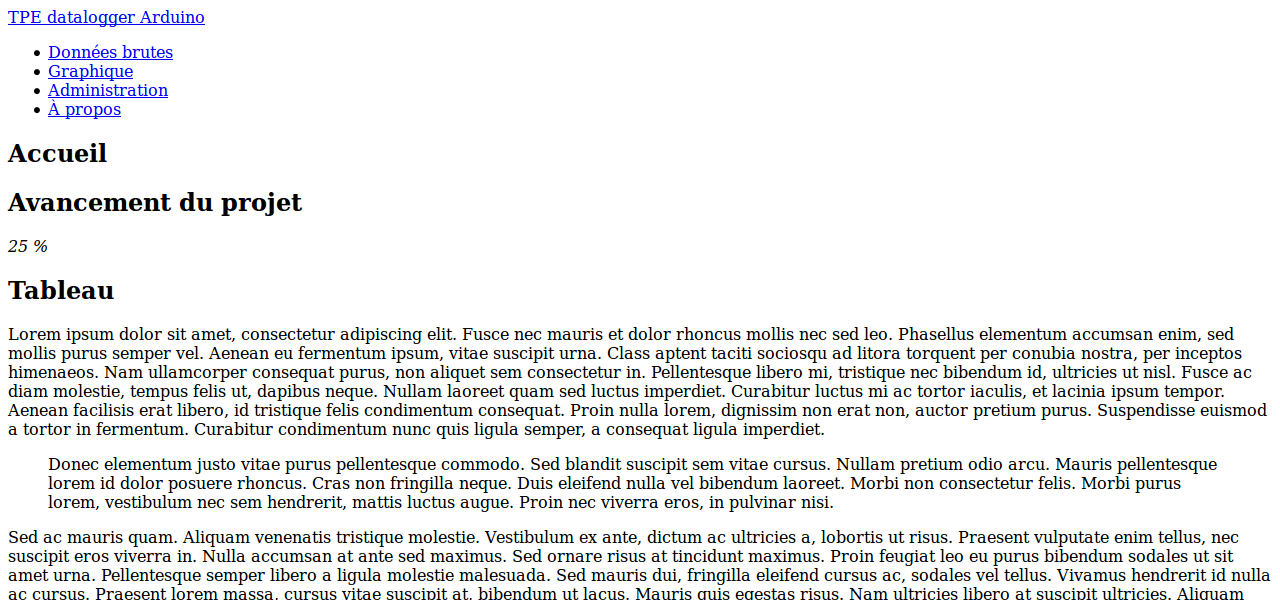
\includegraphics[width=.9\linewidth]{Images/Site_sans_CSS}
	\end{minipage}%
	\begin{minipage}{.5\linewidth}
		\centering
		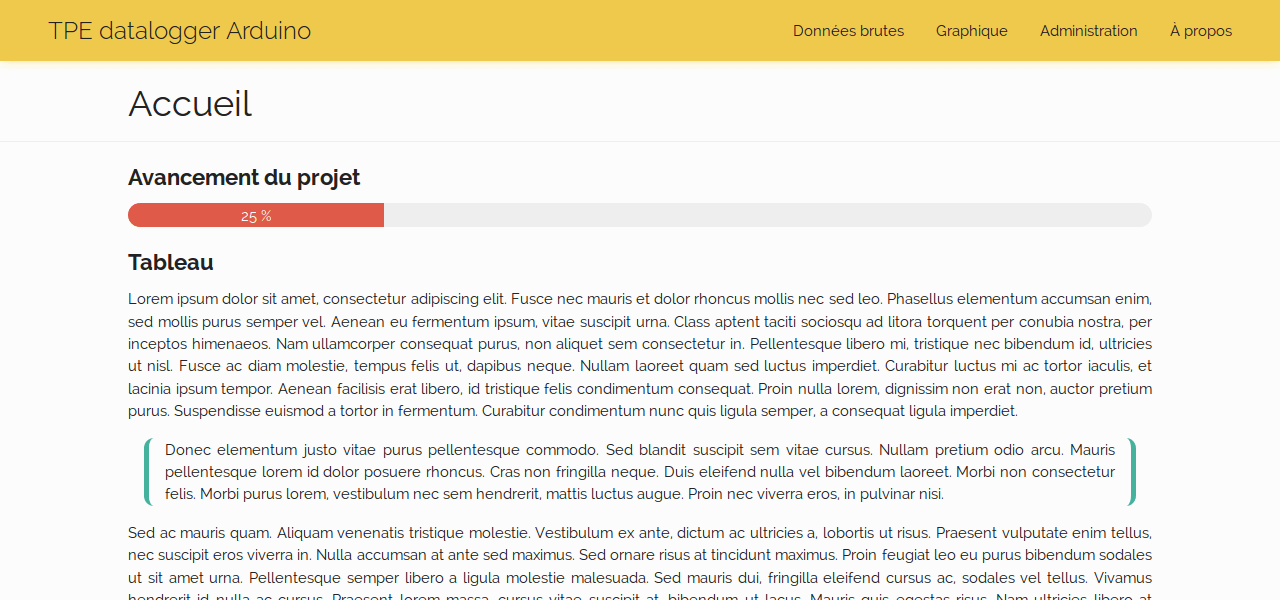
\includegraphics[width=.9\linewidth]{Images/Site_avec_CSS}
	\end{minipage}
	\caption{Notre site sans et avec le CSS}
\end{figure}

\subsection{Partie dynamique : PHP}

Mais notre site a besoin d'être dynamique, de changer au cours du temps. Pour cela, nous utilisons le langage PHP. Ce langage s'exécute sur le serveur que nous avons mis en place (voir chapitre \ref{chapitre:serveur}) à l'inverse du HTML et du CSS qui s'exécute du côté client.

Un code PHP se trouve entre \verb-<?php- et \verb-?>-. À l'intérieur, nous pouvons mettre des variables, des structures conditionnelles, des boucles, etc. Le code suivant affiche un simple texte.
\FichierCode{PHP}{Codes/PHP/Exemple.php}

Le PHP sert à générer du code HTML statique. Ce langage va nous servir à ajouter et à récupérer les différentes données dans la base MySQL.

\subsubsection{Exécuter des requêtes SQL avec PHP}

Pour communiquer avec une base MySQL, nous utilisons un module PHP nommé PDO. Celui-ci facilite les requêtes. Le code suivant liste les données de la table \verb-datalog_meteo- présentée dans la partie précédente.
\FichierCode{PHP}{Codes/PHP/Exemple_PDO.php}
Le résultat généré est alors visible dans un navigateur.
\FichierCode{Text}{Codes/PHP/Resultat_PDO.txt}

\section{Ajout des données par l'Arduino}
\label{section:script-arduino}

Afin que l'Arduino puisse transmettre ces données à la base, il va falloir créer un script qui va être chargé par celui-ci (voir section \ref{section:url-arduino}). Ce script va recevoir les arguments passés dans l'URL. Il y aura trois arguments :
\begin{itemize}
	\item \verb-temperature- contiendra la température ;
	\item \verb-pression- contiendra la pression ;
	\item et \verb-mdp- contiendra le mot de passe pour sécuriser l'accès à la base (ici, \verb-123-).
\end{itemize}
Ainsi, nous créons un fichier \verb-arduino.php- à la racine du site. Le fichier \verb-sql.php- qui contient tout le code pour accéder à la base MySQL est disponible en annexe.
\FichierCode{PHP}{Codes/PHP/Arduino.php}

\section{Récupération des données}

L'objectif principal du site est de proposer un tableau de données. À l'aide de PHP, il faut coder une fonction qui crée le tableau recueillant les données venant la base avec un nombre limité de valeurs pour éviter un tableau trop long qui serait illisible.

Il a donc fallu d'abord créer l'en-tête du tableau puis demander à la base d'aller chercher les valeurs. Nous avons donc créé une fonction que nous appellerons sur la page adéquate. Encore une fois, le fichier \verb-connect.php- qui permet la connexion à la base se trouve en annexe.
\FichierCode{HTML+PHP}{Codes/PHP/Tableau.php}

Ainsi, les valeurs s'ajoutent petit à petit dans les cases avec l'heure à laquelle elle ont été prises. Par exemple, en créant une page avec la fonction \verb-afficher_tableau(20)-, nous pourrons voir un tableau des 20 derniers relevés.

\section{Le graphique de données}

Enfin, pour que les données soient plus lisibles, nous avons décidé de créer un graphique. Sur Internet, nous avons repéré Highchart : c'est une bibliothèque JavaScript générant des graphiques vectoriels en HTML.

À partir des démonstrations proposées sur le site de Highchart\footnote{Voir \url{http://www.highcharts.com/demo}.}, nous pouvons créer un graphique pour les températures. Afin de faire apparaître ces courbes, il faut d'abord dessiner les axes (heures en abscisses, température en ordonnées), les graduer et d'afficher la courbe.
\FichierCode{HTML}{Codes/HTML-CSS/Exemple_graphique.html}
Nous pouvons ainsi observer le résultat suivant.

\begin{figure}[!h]
	\centering
	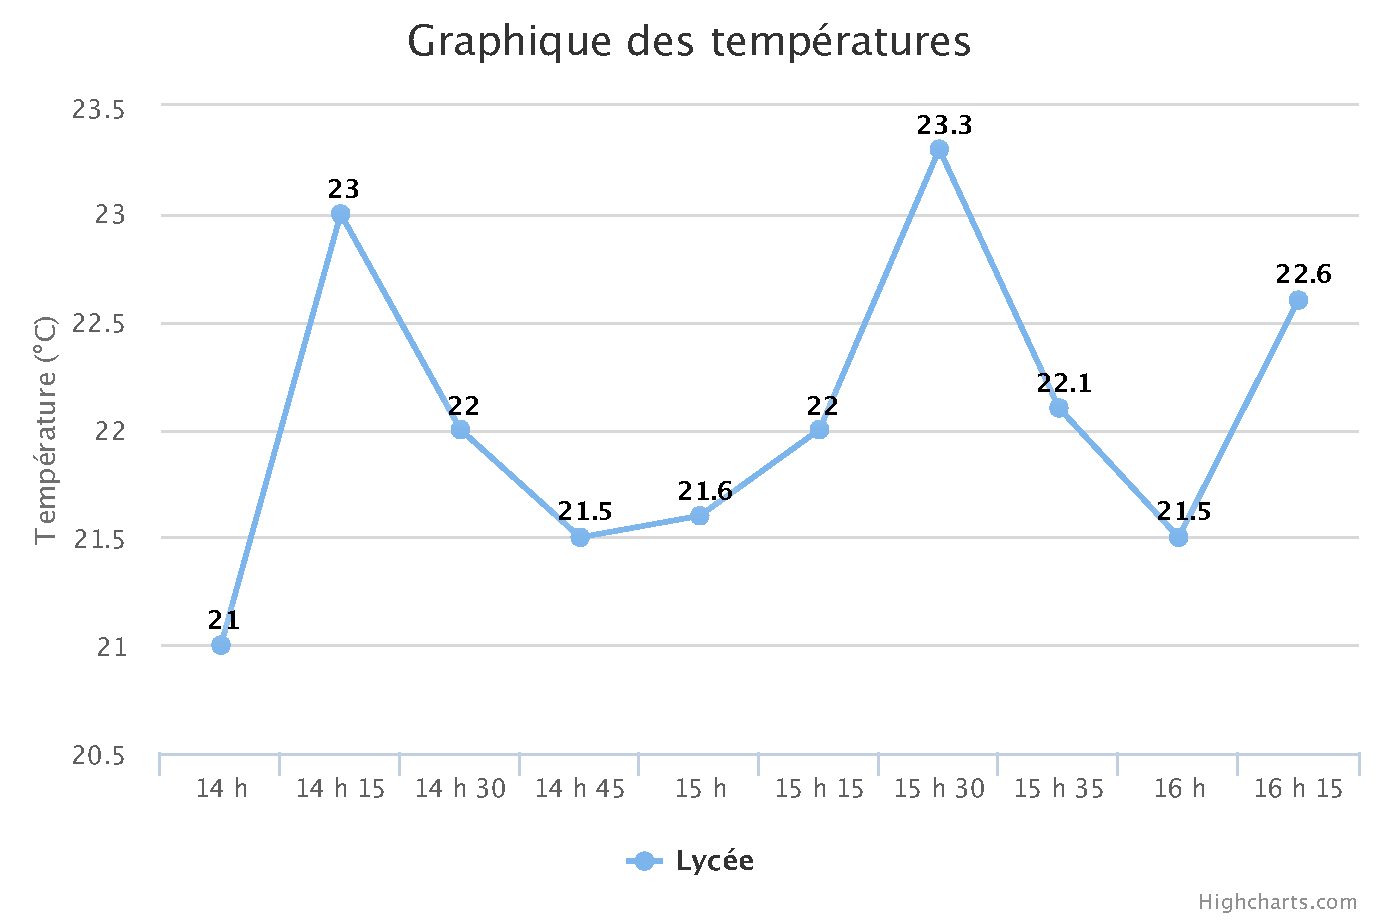
\includegraphics[width=.6\linewidth]{Images/Exemple_graphique}
	\caption{Graphique avec Highchart}
\end{figure}

Il faut donc que nous codions une fonction PHP qui récupère les données et qui les adapte au code pour Highchart. Ce graphique mettra en image l'évolution de la température et de la pression en fonction du temps.

Tout le code du site, un peu long, est disponible en annexe à la page \pageref{code:site}.
